\subsection{Analyse de l'entropie dans Mathematica}
\newcommand{\EntropyGfxScale}{0.8\textwidth}

(Cette partie est parue initialement sur mon blog le 13 mai 2015.
Quelques discussions: \url{https://news.ycombinator.com/item?id=9545276}.)

Il est possible de découper un fichier par blocs, de calculer l'entropie de chacun
d'eux et de dessiner un graphe.
J'ai fais ceci avec Wolfram Mathematica à titre de démonstration et voici le code
source (Mathematica 10):

\begin{lstlisting}[style=custommath]
(* loading the file *)
input=BinaryReadList["file.bin"];

(* setting block sizes *)
BlockSize=4096;BlockSizeToShow=256;

(* slice blocks by 4k *)
blocks=Partition[input,BlockSize];

(* how many blocks we've got? *)
Length[blocks]

(* calculate entropy for each block. 2 in Entropy[] (base) is set with the intention so Entropy[] 
function will produce the same results as Linux ent utility does *)
entropies=Map[N[Entropy[2,#]]&,blocks];

(* helper functions *)
fBlockToShow[input_,offset_]:=Take[input,{1+offset,1+offset+BlockSizeToShow}]
fToASCII[val_]:=FromCharacterCode[val,"PrintableASCII"]
fToHex[val_]:=IntegerString[val,16]
fPutASCIIWindow[data_]:=Framed[Grid[Partition[Map[fToASCII,data],16]]]
fPutHexWindow[data_]:=Framed[Grid[Partition[Map[fToHex,data],16],Alignment->Right]]

(* that will be the main knob here *)
{Slider[Dynamic[offset],{0,Length[input]-BlockSize,BlockSize}],Dynamic[BaseForm[offset,16]]}

(* main UI part *)
Dynamic[{ListLinePlot[entropies,GridLines->{{-1,offset/BlockSize,1}},Filling->Axis,AxesLabel->{"offset","entropy"}],
CurrentBlock=fBlockToShow[input,offset];
fPutHexWindow[CurrentBlock],
fPutASCIIWindow[CurrentBlock]}]
\end{lstlisting}

\subsubsection{Base de données GeoIP de FAI}

\myindex{GeoIP}
Commençons avec le fichier \href{https://www.maxmind.com/en/geoip-demo}{GeoIP} (qui
assigne un FAI au bloc d'adresses IP).
Ce fichier binaire \emph{GeoIPISP.dat} a plusieurs tables (qui sont peut-être les
intervalles d'adresses IP) plus quelques blobs de texte à la fin du fichier (contenant
les noms des FAI).

Lorsque je le charge dans Mathematica, je vois ceci:

\begin{figure}[H]
\centering
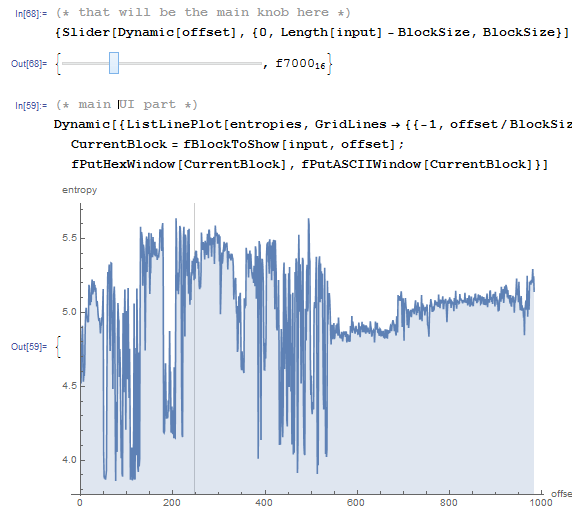
\includegraphics[width=\EntropyGfxScale]{ff/entropy/geoipisp11.png}
\end{figure}

\begin{figure}[H]
\centering
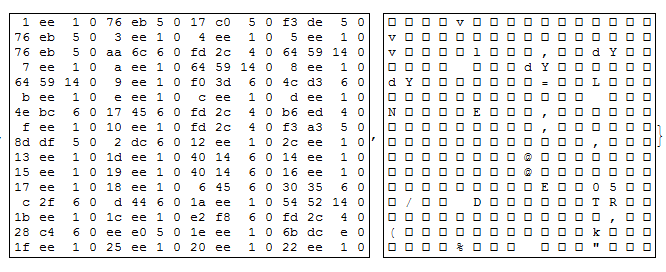
\includegraphics[width=\EntropyGfxScale]{ff/entropy/geoipisp12.png}
\end{figure}


Il y a deux parties dans le graphe: la première est un peu chaotique, la seconde
est plus régulière.

0 sur l'axe vertical du graphe signifie l'entropie la plus basse (les données
qui peuvent être compressée très fortement, \emph{ordonnées} en d'autres mots) et 8
est la plus haute (ne peuvent pas être compressées du tout, \emph{chaotique}
ou \emph{aléatoires} en d'autres mots).
Pourquoi 0 et par 8? 0 signifie 0 bits par octet (l'octet en tant que conteneur
n'est pas rempli du tout) et 8 signifie 8 bits par octet, i.e., l'octet comme
conteneur est complètement rempli d'information.

Donc, je mets le curseur pour pointer sur le milieu du premier bloc, et je vois clairement
des tableaux d'entiers 32-bit.
Maintenant je mets le curseur au milieu du second bloc et je vois un texte en anglais:

\begin{figure}[H]
\centering
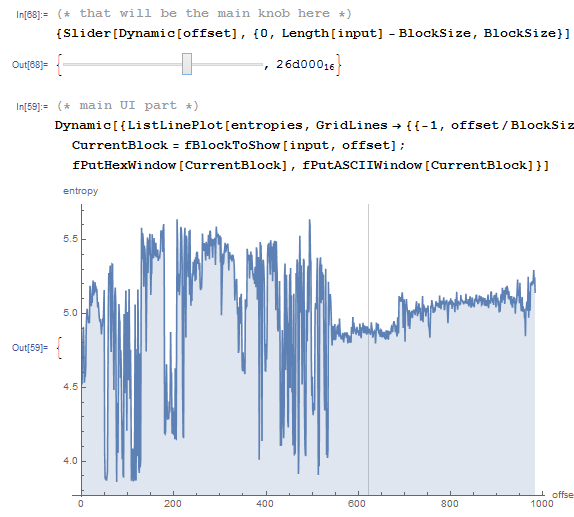
\includegraphics[width=\EntropyGfxScale]{ff/entropy/geoipisp21.png}
\end{figure}

\begin{figure}[H]
\centering
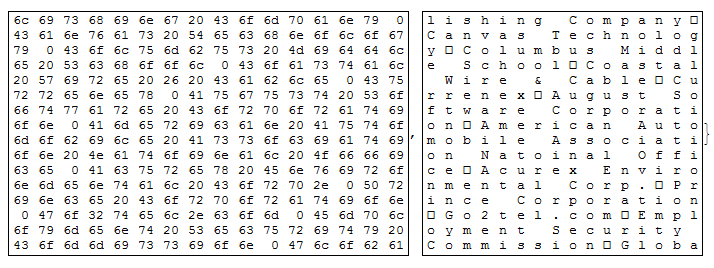
\includegraphics[width=\EntropyGfxScale]{ff/entropy/geoipisp22.png}
\end{figure}


En effet, ceci sont les noms des FAIs.
Donc, l'entropie de textes en anglais est 4.5-5 bits par octet? Oui, quelque chose
comme ça.
Wolfram Mathematica comprend quelques corpus de littérature anglaise bien connu,
et nous pouvons voir l'entropie de sonnets de Shakespeare:

\begin{lstlisting}[style=custommath]
In[]:= Entropy[2,ExampleData[{"Text","ShakespearesSonnets"}]]//N
Out[]= 4.42366
\end{lstlisting}

4,4 est proche de ce que nous obtenons ()4.7-5.3).
Bien sûr, les textes de la littérature anglaise classique sont quelques peu différents
des noms des FAIs et autres texte en anglais que nous pouvons trouver dans des fichiers
binaires (débogage/trace/messages d'erreur), mais cette valeur est proche.

\subsubsection{Firmware TP-Link WR941 }

Pour l'exemple suivant, j'ai pris le firmware du routeur TP-Link WR941:

\begin{figure}[H]
\centering
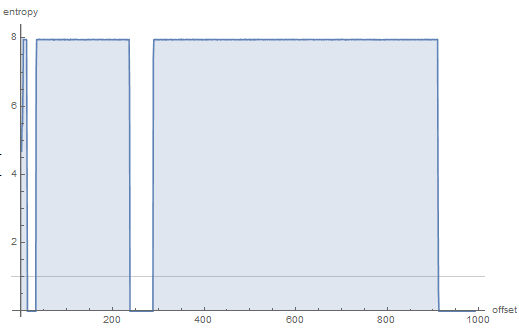
\includegraphics[width=\EntropyGfxScale]{ff/entropy/tplink.png}
\end{figure}


Nous voyons ici 3 blocs avec des vides.
Puis le premier bloc avec une haute entropie (démarrant à l'adresse 0) est petit,
le second (adresse quelque part en 0x22000) et plus grand et le troisième
(adresse 0x123000) est le plus grand.
Je ne peux pas être certain de l'entropie du premier bloc, mais le 2-ème et le 3-ème
ont une entropie très haute, signifiant que ces blocs sont soit compressés et/ou
chiffrés.

\myindex{Binwalk}
J'ai essayé \href{http://binwalk.org/}{binwalk} pour ce fichier de firmware:

\begin{lstlisting}
DECIMAL       HEXADECIMAL     DESCRIPTION
--------------------------------------------------------------------------------
0             0x0             TP-Link firmware header, firmware version: 0.-15221.3, image version: "", product ID: 0x0, product version: 155254789, kernel load address: 0x0, kernel entry point: 0x-7FFFE000, kernel offset: 4063744, kernel length: 512, rootfs offset: 837431, rootfs length: 1048576, bootloader offset: 2883584, bootloader length: 0
14832         0x39F0          U-Boot version string, "U-Boot 1.1.4 (Jun 27 2014 - 14:56:49)"
14880         0x3A20          CRC32 polynomial table, big endian
16176         0x3F30          uImage header, header size: 64 bytes, header CRC: 0x3AC66E95, created: 2014-06-27 06:56:50, image size: 34587 bytes, Data Address: 0x80010000, Entry Point: 0x80010000, data CRC: 0xDF2DBA0B, OS: Linux, CPU: MIPS, image type: Firmware Image, compression type: lzma, image name: "u-boot image"
16240         0x3F70          LZMA compressed data, properties: 0x5D, dictionary size: 33554432 bytes, uncompressed size: 90000 bytes
131584        0x20200         TP-Link firmware header, firmware version: 0.0.3, image version: "", product ID: 0x0, product version: 155254789, kernel load address: 0x0, kernel entry point: 0x-7FFFE000, kernel offset: 3932160, kernel length: 512, rootfs offset: 837431, rootfs length: 1048576, bootloader offset: 2883584, bootloader length: 0
132096        0x20400         LZMA compressed data, properties: 0x5D, dictionary size: 33554432 bytes, uncompressed size: 2388212 bytes
1180160       0x120200        Squashfs filesystem, little endian, version 4.0, compression:lzma, size: 2548511 bytes, 536 inodes, blocksize: 131072 bytes, created: 2014-06-27 07:06:52
\end{lstlisting}

\myindex{LZMA}
En effet: il y a des choses au début, mais deux larges blocs compressés LZMA
commencent en 0x20400 et 0x120200.
Ce sont en gros les adresses que nous avons vu dans Mathematica.
Oh, à propos, binwalk peut aussi afficher l'entropie (option \TT{-E}):

\begin{lstlisting}
DECIMAL       HEXADECIMAL     ENTROPY
--------------------------------------------------------------------------------
0             0x0             Falling entropy edge (0.419187)
16384         0x4000          Rising entropy edge (0.988639)
51200         0xC800          Falling entropy edge (0.000000)
133120        0x20800         Rising entropy edge (0.987596)
968704        0xEC800         Falling entropy edge (0.508720)
1181696       0x120800        Rising entropy edge (0.989615)
3727360       0x38E000        Falling entropy edge (0.732390)
\end{lstlisting}

Les fronts ascendants correspondent à des fronts ascendants de blocs sur notre graphe.
Les fronts descendants sont des points où des espaces vides commencent.

Binwalk peut aussi générer un graphe PNG (\TT{-E -J}):

\begin{figure}[H]
\centering
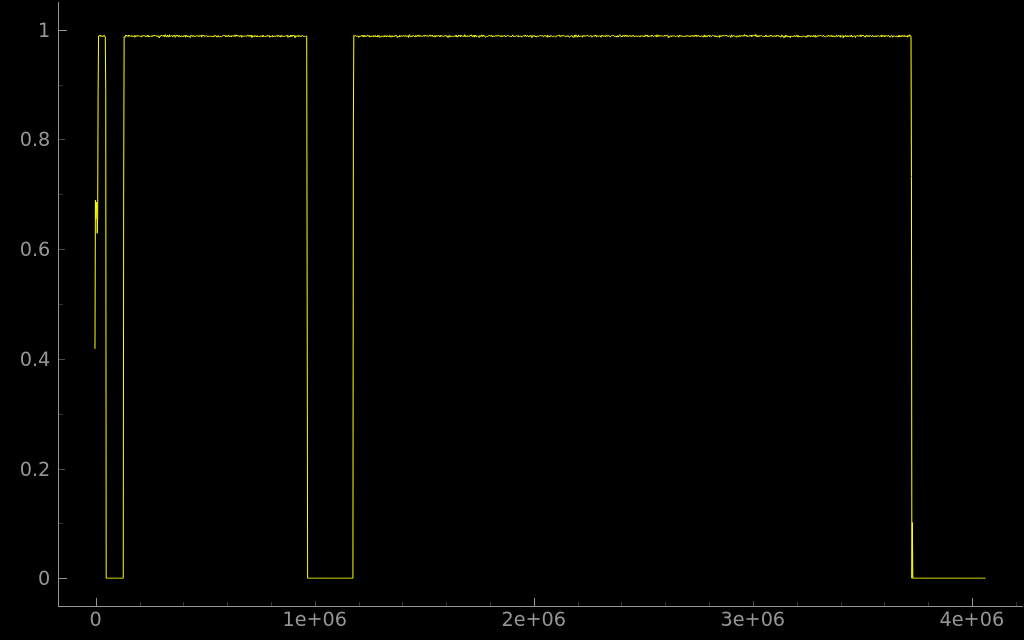
\includegraphics[width=\EntropyGfxScale]{ff/entropy/tplink_binwalk.png}
\end{figure}


Que pouvons-nous dire à propos de ces espaces vides? En regardant dans un éditeur hexadécimal,
nous voyons qu'ils sont simplement remplis avec des octets à 0xFF.
Pourquoi les développeurs les ont-ils mises?
Peut-être parce qu'ils n'ont pas pu calculer précisément la taille des blocs compressés,
et leurs ont donc alloué de l'espace avec une marge.

\subsubsection{Notepad}

\myindex{Notepad}

Un autre exemple est notepad.exe que j'ai pris dans Windows 8.1:

\begin{figure}[H]
\centering
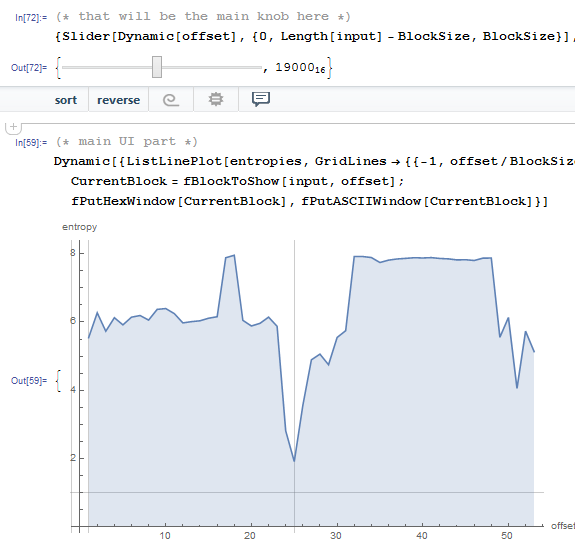
\includegraphics[width=\EntropyGfxScale]{ff/entropy/notepad11.png}
\end{figure}

\begin{figure}[H]
\centering
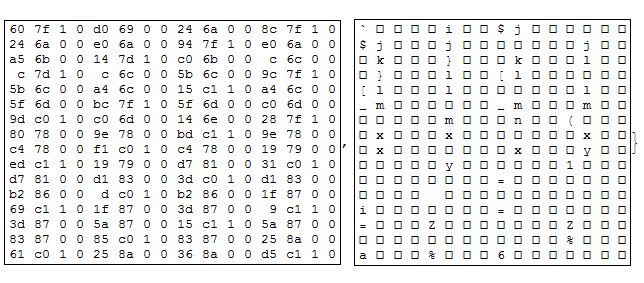
\includegraphics[width=\EntropyGfxScale]{ff/entropy/notepad12.png}
\end{figure}


Il y a un creux à $\approx 0x19000$ (offset absolu dans le fichier).
J'ai ouvert le fichier exécutable dans un éditeur hexadécimal et trouvé des tables
d'imports (qui ont une entropie plus basse que le code x86-64 dans la première moitié
du graphe).

Il y a aussi un bloc avec une grande entropie qui démarre $\approx 0x20000$:

\begin{figure}[H]
\centering
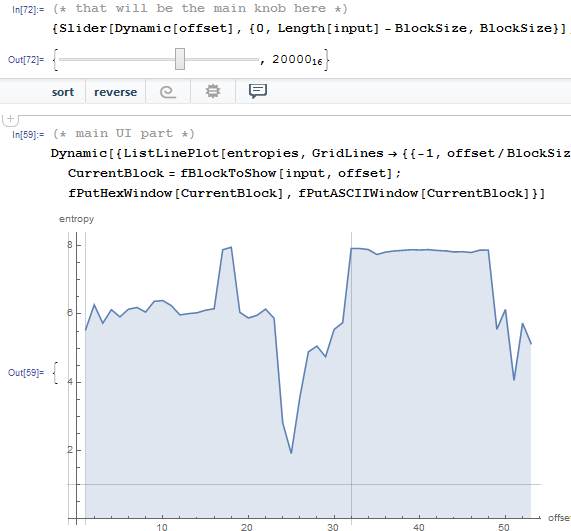
\includegraphics[width=\EntropyGfxScale]{ff/entropy/notepad21.png}
\end{figure}

\begin{figure}[H]
\centering
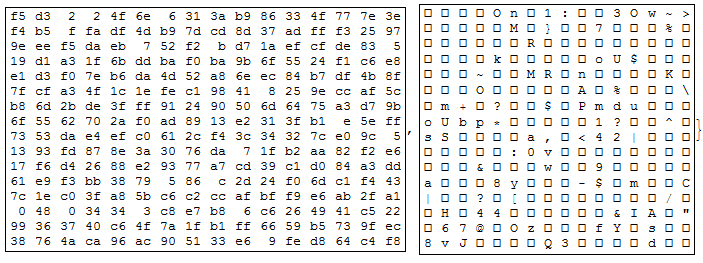
\includegraphics[width=\EntropyGfxScale]{ff/entropy/notepad22.png}
\end{figure}


\myindex{PNG}
Dans un éditeur hexadécimal je peux y voir un fichier PNG, inséré dans la section
ressource du fichier PE (c'est une grosse image de l'icône de notepad).
Les fichiers PNG sont compressés, en effet.

\subsubsection{Dashcam sans marque}

Maintenant l'exemple le plus avancé dans cette partie est le firmware d'une dashcam
sans marque que j'ai reçu d'un ami:

\begin{figure}[H]
\centering
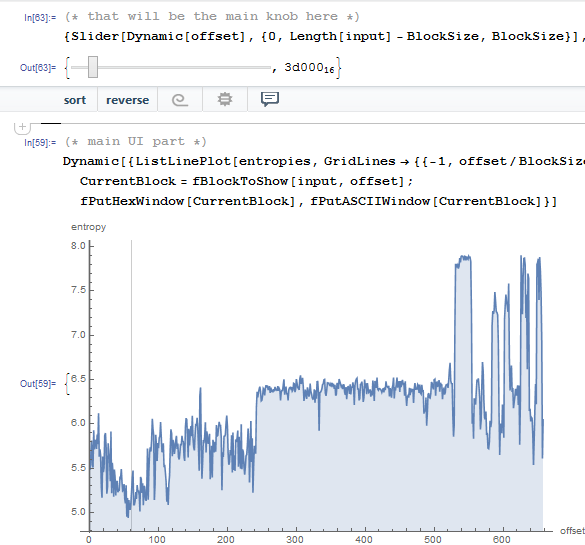
\includegraphics[width=\EntropyGfxScale]{ff/entropy/dashcam_text1.png}
\end{figure}

\begin{figure}[H]
\centering
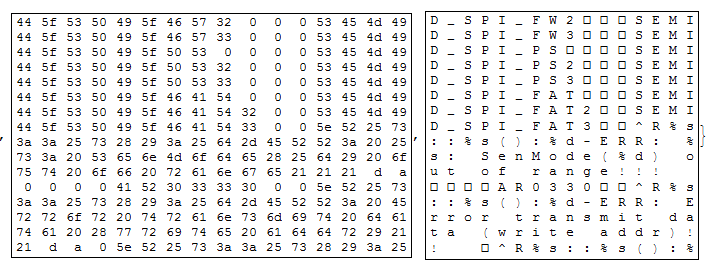
\includegraphics[width=\EntropyGfxScale]{ff/entropy/dashcam_text2.png}
\end{figure}


La creux au tout début est un texte en anglais: messages de débogage.
\myindex{MIPS}
J'ai vérifié différents \ac{ISA}s et j'ai trouvé que le premier tiers du fichier
complet (avec le segment de texte dedans) est en fait du code MIPS (petit-boutiste).

Par exemple, ceci est une fonction épilogue MIPS très typique:

\begin{lstlisting}[style=customasmMIPS]
ROM:000013B0                 move    $sp, $fp
ROM:000013B4                 lw      $ra, 0x1C($sp)
ROM:000013B8                 lw      $fp, 0x18($sp)
ROM:000013BC                 lw      $s1, 0x14($sp)
ROM:000013C0                 lw      $s0, 0x10($sp)
ROM:000013C4                 jr      $ra
ROM:000013C8                 addiu   $sp, 0x20
\end{lstlisting}

D'après notre graphe nous pouvons voir que le code MIPs a une entropie de 5-6 bits
par octet.
En effet, j'ai mesuré une fois l'entropie de différents \ac{ISA}s et j'ai obtenu
ces valeurs:

\begin{itemize}
\item x86: section .text du fichier ntoskrnl.exe de Windows 2003: 6.6
\item x64: section .text du fichier ntoskrnl.exe de Windows 7 x64: 6.5
\item ARM (mode thumb), Angry Birds Classic: 7.05
\item ARM (mode ARM) Linux Kernel 3.8.0: 6.03
\item MIPS (little endian), section .text du fichier user32.dll de Windows NT 4: 6.09
\end{itemize}

Donc l'entropie du code exécutable est plus grande que du texte en anglais, mais
peut encore être compressé.

Maintenant le second tiers qui commence en 0xF5000. Je ne sais pas ce que c'est.
J'ai essayé différents \ac{ISA}s mais sans succès.
L'entropie de ce bloc semble encore plus régulière que celui de l'exécutable.
Peut-être des sortes de données?

\myindex{JPEG}
Il y a aussi un pic en $\approx 0x213000$.
Je l'ai vérifié dans un éditeur hexadécimal et j'y ai trouvé un fichier JPEG (qui
est, bien sûr, compressé)!
Je ne sais pas ce qu'il y a à la fin.
Essayons Binwalk pour ce fichier:

\begin{lstlisting}
% binwalk FW96650A.bin 

DECIMAL       HEXADECIMAL     DESCRIPTION
--------------------------------------------------------------------------------
167698        0x28F12         Unix path: /15/20/24/25/30/60/120/240fps can be served..
280286        0x446DE         Copyright string: "Copyright (c) 2012 Novatek Microelectronic Corp."
2169199       0x21196F        JPEG image data, JFIF standard 1.01
2300847       0x231BAF        MySQL MISAM compressed data file Version 3

% binwalk -E FW96650A.bin 

DECIMAL       HEXADECIMAL     ENTROPY
--------------------------------------------------------------------------------
0             0x0             Falling entropy edge (0.579792)
2170880       0x212000        Rising entropy edge (0.967373)
2267136       0x229800        Falling entropy edge (0.802974)
2426880       0x250800        Falling entropy edge (0.846639)
2490368       0x260000        Falling entropy edge (0.849804)
2560000       0x271000        Rising entropy edge (0.974340)
2574336       0x274800        Rising entropy edge (0.970958)
2588672       0x278000        Falling entropy edge (0.763507)
2592768       0x279000        Rising entropy edge (0.951883)
2596864       0x27A000        Falling entropy edge (0.712814)
2600960       0x27B000        Rising entropy edge (0.968167)
2607104       0x27C800        Rising entropy edge (0.958582)
2609152       0x27D000        Falling entropy edge (0.760989)
2654208       0x288000        Rising entropy edge (0.954127)
2670592       0x28C000        Rising entropy edge (0.967883)
2676736       0x28D800        Rising entropy edge (0.975779)
2684928       0x28F800        Falling entropy edge (0.744369)
\end{lstlisting}

Oui, il trouve un fichier JPEG et même des données MySQL!
Mais je ne suis pas certain que ça soit vrai---je ne l'ai pas encore vérifié.

\myindex{clusterization}
Il est aussi intéressant d'essayer la clusterisation dans Mathematica:

\begin{figure}[H]
\centering
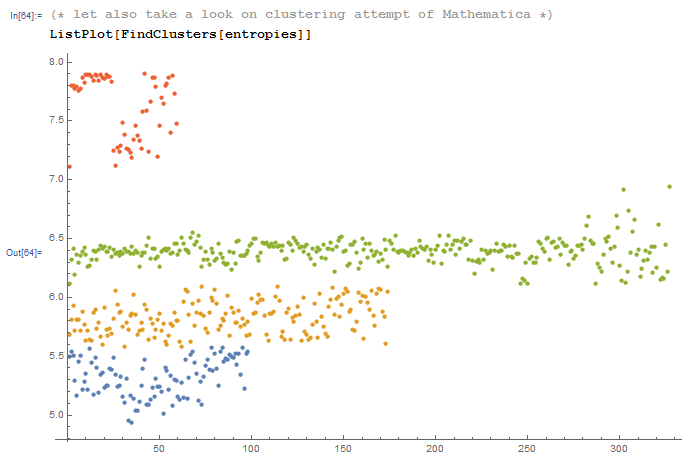
\includegraphics[width=\EntropyGfxScale]{ff/entropy/dashcam_clusters.png}
\end{figure}


Ceci est un exemple de la façon dont Mathematica groupe des valeurs d'entropie diverses
dans des groupes distincts.
En effet, c'est quelque chose de plausible.
Les points bleus dans l'intervalle 5.0-5.5 sont probablement relatif à du texte en
anglais,
Les points jaunes dans 5.5-6 sont du code MIPS. Beaucoup de points verts dans 6.0-6.5
sont dans le second tiers non identifié.
Les points orange proches de 8.0 sont relatifs au fichier JPEG compressé.
D'autres points orange sont probablement relatif à la fin du firmware (données inconnues
pour nous).

\subsubsection{Liens}

Fichiers binaires utilisés dans cette partie: \\
\url{\RepoURL/ff/entropy/files/}.\\
Fichier notebook Wolfram Mathematica: \\
\url{\RepoURL/ff/entropy/files/binary_file_entropy.nb} \\
(toutes les cellules doivent être évaluées pour que ça commence à fonctionner).
